\chapter{Apéndice}\label{ch:Ap}

\section{Demostraciones del texto}
\subsection{Solución de un sistema lineal}
Se anexa la demostración al \textbf{Teorema 1} [\ref{teo:Solgral}]:
\begin{proof}
	Se propone la función general $X(t)=e^{\lambda t}\vec{v}_0$. Entonces derivamos la función con respecto del tiempo
	\begin{align*}
		\dot{X}(t) &= \lambda e^{\lambda t}\vec{v}_0\\
				   &= e^{\lambda t}(\lambda\vec{v}_0)\\
				   &= e^{\lambda t}(A\vec{v}_0)		\\
				   &= A(e^{\lambda t}\vec{v}_0)\\
				   &= AX(t)
	\end{align*}
\end{proof}

\subsection{Solución de la ecuación logística}\label{sec:SolEqLogistica}

La ecuación logística (\ref{eqn:EqLogistica}) es de las pocas ecuaciones no lineales de las que podemos hallar una solución analítica única. A continuación nos adentraremos a hallar dicha solución. Reescribimos la ecuación de la siguiente manera
$$\frac{dN}{dt}=\frac{rN(K-N)}{K}$$
se utiliza la separación de variables para poder resolver la ecuación, re acomodando nos queda como
$$\frac{KdN}{N(K-N)}=rdt\qquad\Longleftrightarrow\qquad \int\frac{KdN}{N(K-N)}=\int rdt$$
El lado izquierdo lo resolvemos por fracciones parciales, se encomienda al lector comprobar que la siguiente igualdad es verdadera
$$\frac{K}{N(N-K)}=\frac{1}{N}+\frac{1}{K-N}$$
entonces las integrales ya resueltas nos quedan de la siguiente manera
\begin{align*}
	\ln N-\ln(K-N)&=rt+c \\
	\ln\left (\frac{N}{K-N}\right ) &= rt+c\\
	\frac{N}{K-N}&=e^{rt+c}\\
	N&=(K-N)Ce^{rt}\\
	N(1+Ce^{rt})&=KCe^{rt}\\
	N(t)&=\frac{KCe^{rt}}{1+Ce^{rt}}
\end{align*}
Resolviendo el problema de condición inicial se establece que para $t=0$ se tiene $N(0)=N_0$, por tanto la constante $C$ nos queda como
$$C=\frac{N_0}{K-N_0}$$
Finalmente reajustando y acomodando términos, la solución de la ecuación logística es:
\begin{equation}\label{eqn:SolEqLogistica}
	N(t)=\frac{KN_0e^{rt}}{(K-N_0)+N_0e^{rt}}
\end{equation}
Comparado con la solución numérica se ve de la siguiente forma
\begin{figure}[h!]
	\centering
	\includegraphics[scale=0.23]{../Imagenes/Ecuacion Logistica Analítica}
	\caption{Ecuación logística con una tasa de crecimiento $r=2$ y una capacidad de carga $K=10$, se grafica para las mismas condiciones iniciales; (\textbf{A}) Solución analítica. (\textbf{B}) Solución numérica.}
	\label{fig:EcuacionLogisticaAnalitica}
\end{figure}
\newpage
\subsection{Solución del sistema presa-depredador}\label{sec:SolPresaDepredador}

El sistema (\ref{eqn:PresaDepredador}) tiene la dicha de poderse resolver de forma analítica al igual que la ecuación logística y se verá a continuación el procedimiento. Para ello definimos la siguiente regla de la cadena para $y(t)$
$$\frac{dy}{dt} = \frac{dy}{dx}\cdot\frac{dx}{dt}\qquad\Longleftrightarrow\qquad\frac{dy}{dx}=\frac{\frac{dy}{dt}}{\frac{dx}{dt}}$$
sustituyendo las ecuaciones de (\ref{eqn:PresaDepredador}) en $\frac{dy}{dx}$ se tiene
\begin{align*}
	\frac{dy}{dx}&=\frac{\delta xy-\gamma y}{\alpha x-\beta xy}  \\
\end{align*}
Se factoriza lo necesario y se aplica separación de variables para poder integrar las ecuaciones y hallar las soluciones
\begin{align*}
	x(\alpha-\beta y)\, dy &= y(\delta x-\gamma)\, dx\\
	\int \frac{\alpha-\beta y}{y}\, dy &= \int \frac{\delta x-\gamma}{x}\, dx \\
\end{align*}
al integrar finalmente tenemos la solución implícita:
\begin{equation}\label{eqn:CurvasNivelPD}
	f(x,y)=\alpha\ln y+\gamma\ln x-\beta y- \delta x=c
\end{equation}
Ahora veamos las curvas de nivel de la solución analítica en contraste con el espacio fase generado a través de las ecuaciones de (\ref{eqn:PresaDepredador}):
\begin{figure}[h!]
	\centering
	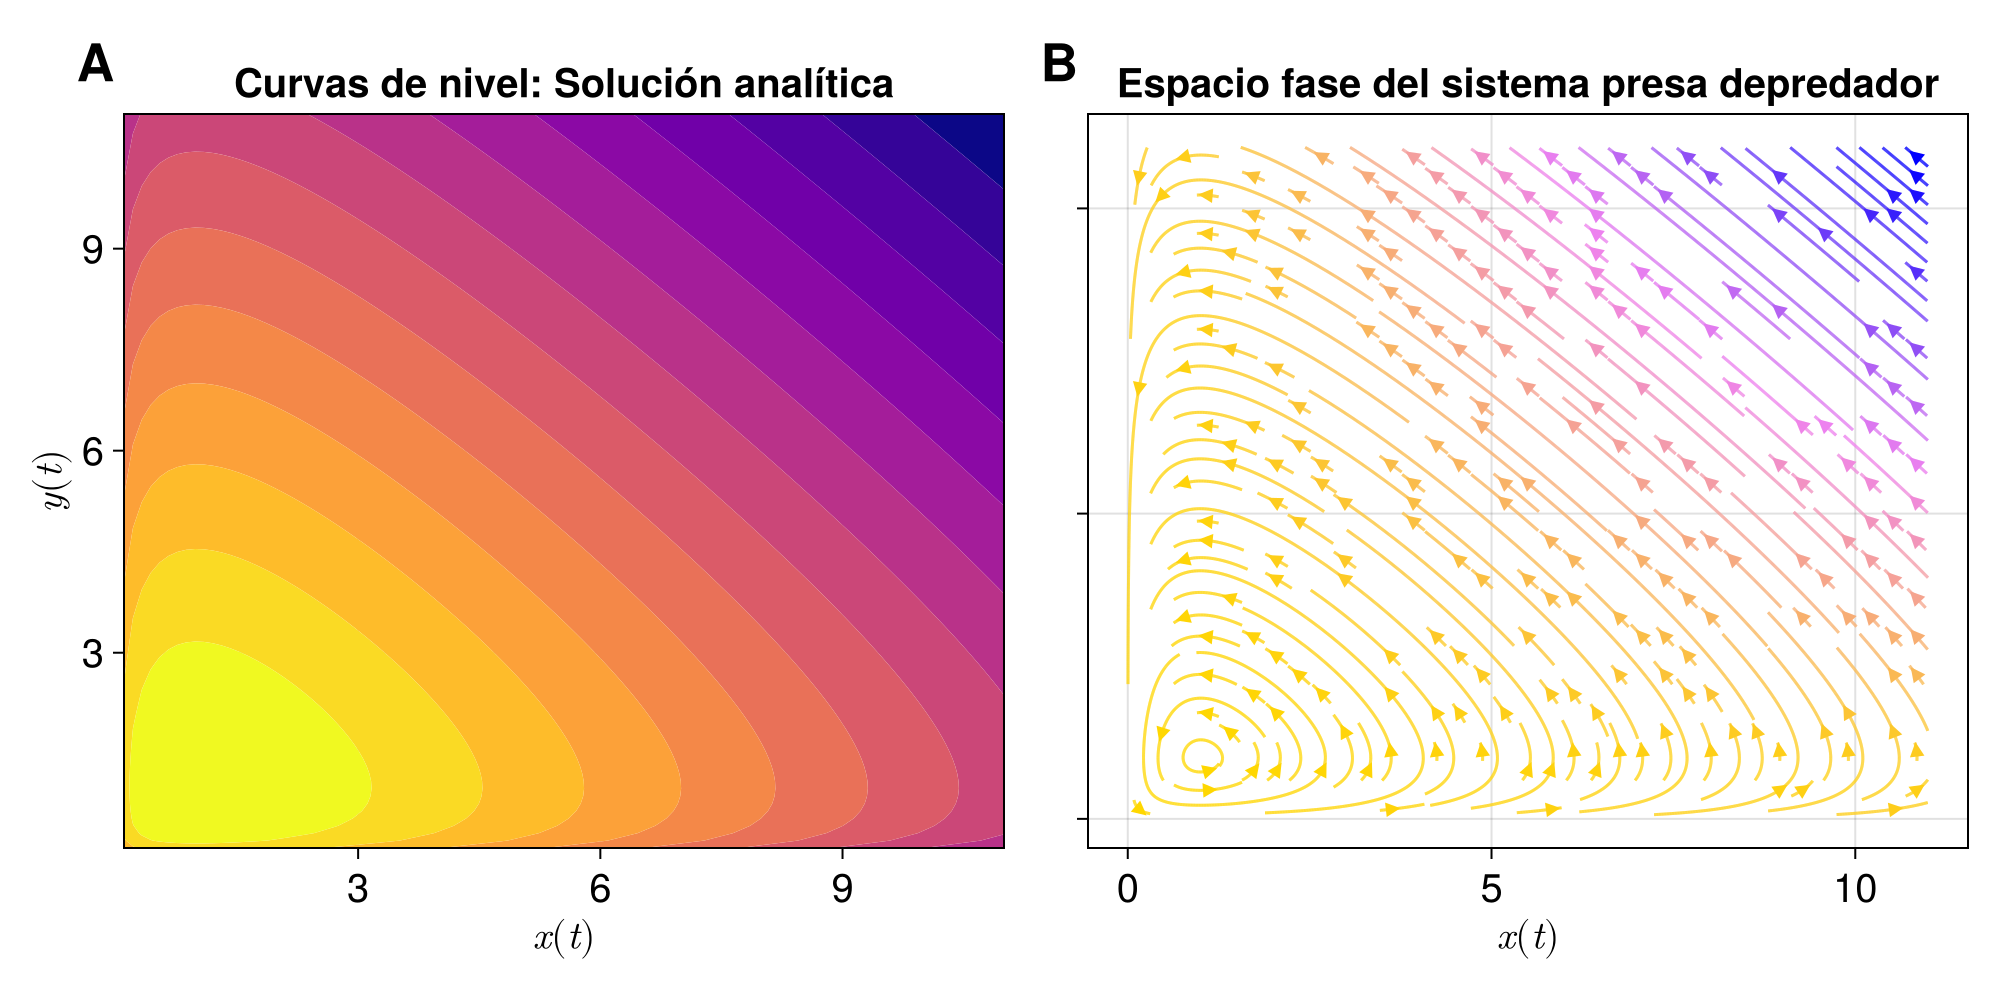
\includegraphics[scale=0.22]{../Imagenes/Curvas de nivel PD}
	\caption{(\textbf{A}) Curvas de nivel utilizando la solución analítica (\ref{eqn:CurvasNivelPD}). (\textbf{B}) Espacio fase generado a partir de las ecuaciones de (\ref{eqn:PresaDepredador}) integrando con RK4.}
	\label{fig:CurvasNivelPD}
\end{figure}
\newpage
Por último realicemos una rápida comparación entre los métodos de integración de RK4 y Euler para poder visualizar la razón principal por la que se ha escogido RK4 como método de integración para los sistemas no lineales de esta tesis.
\begin{figure}[h!]
	\centering
	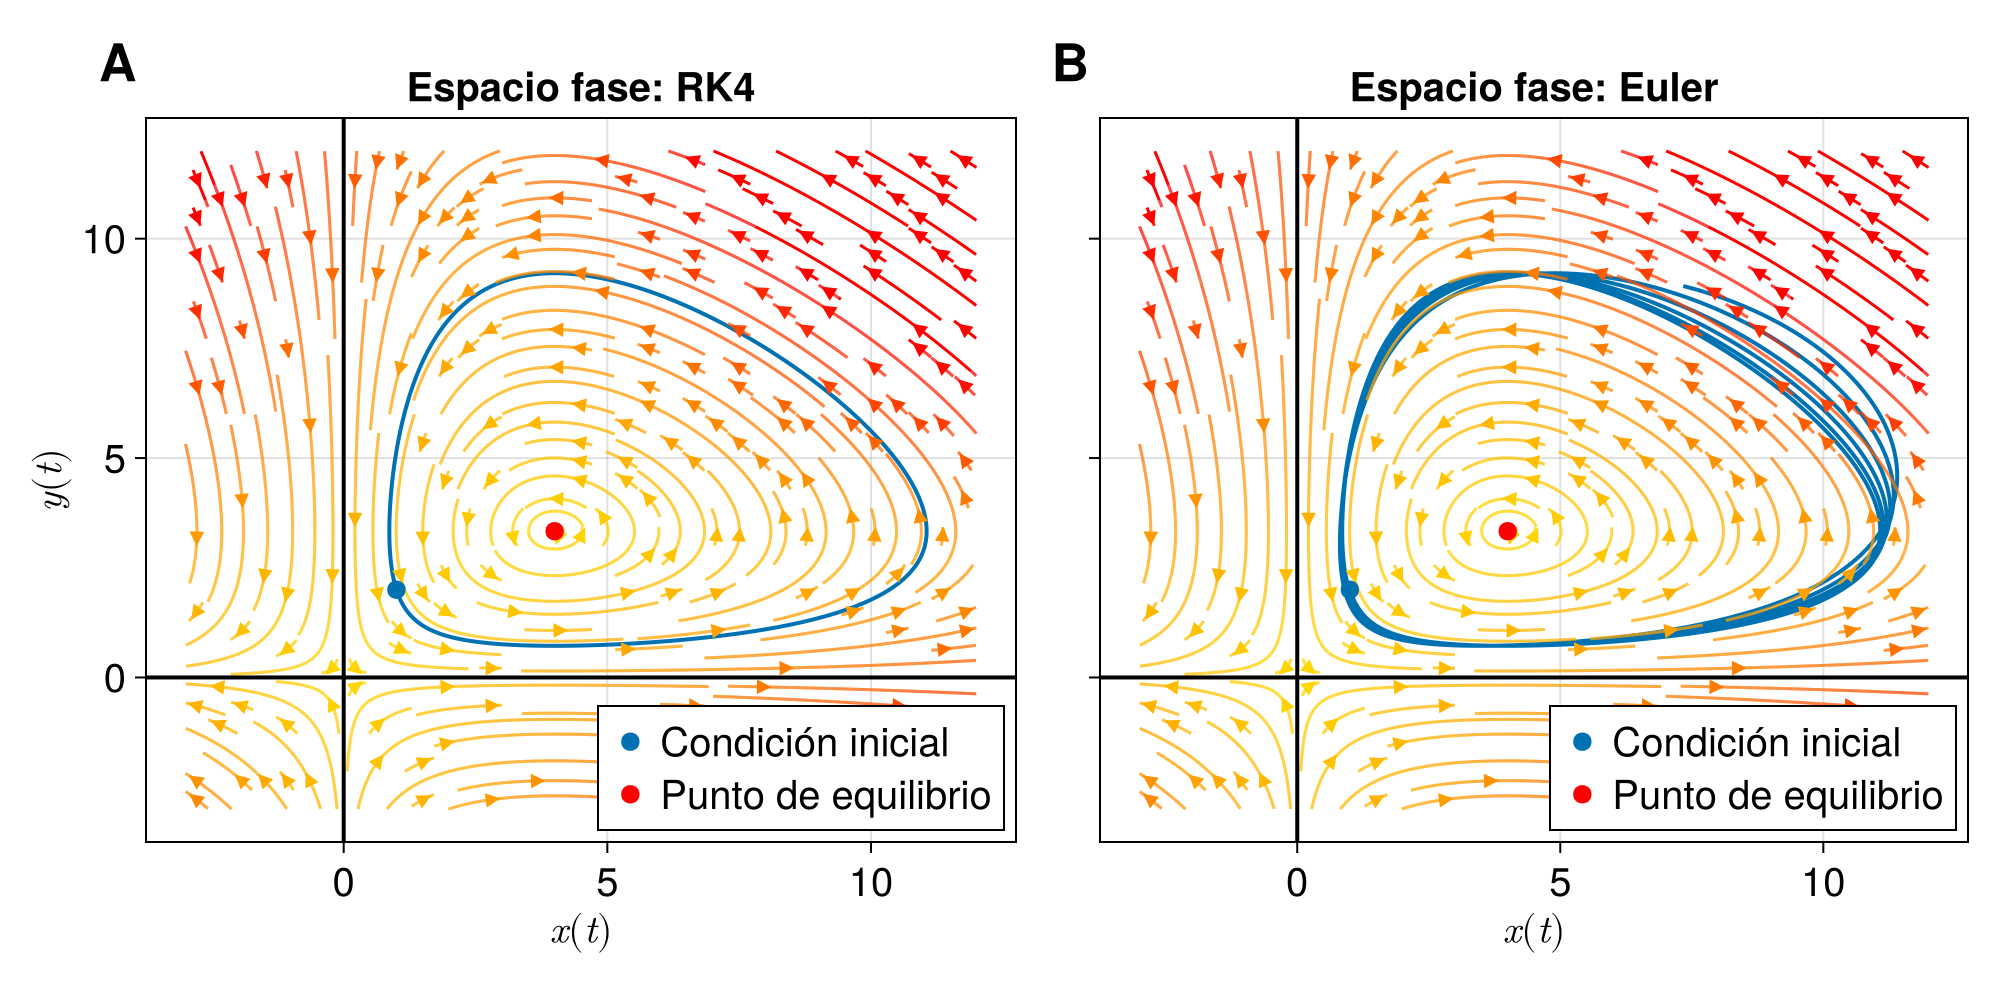
\includegraphics[scale=0.23]{../Imagenes/RK4vsEuler}
	\caption{En ambos ejemplos se integró para $t\in[0,20]$ con un paso de integración de $h=0.01$. (\textbf{A}) Integración del sistema (\ref{eqn:EgPresaDepredador}) con el método de Runge-Kutta de orden 4. (\textbf{B}) Integración del sistema (\ref{eqn:EgPresaDepredador}) con el método de Euler.}
	\label{fig:Rk4vsEuler}
\end{figure}

Para fines prácticos, en la siguiente sección se introducen la implementación de ambos métodos en el lenguaje de programación \julia.

\section{Algoritmos y códigos}

\subsection{Códigos para generar imágenes}
El trabajo presente se ha realizado bajo algoritmos hecho en el lenguaje de programación \julia. En esta sección como en otras se estará anexando código en referencia a elementos presentes en el cuerpo de la tesis. Se anexa código de las figuras de los espacios fase de la sección (\ref{sec:Espacios fase}). Cabe mencionar que el motor de graficación utilizado es \href{https://github.com/JuliaPlots/CairoMakie.jl}{\texttt{CairoMakie.jl}}\footnote{citar} que es ampliamente utilizado para publicaciones científicas por su elegancia, estética y estilo. Se espera que con los bloques de códigos anexados se pueda dar una idea de su uso para su implementación propia del lector.\\
\\
\subsubsection{Espacios fase}
El bloque de código (\ref{al:EspaciosFase}) funciona para generar la Figura (\ref{fig:EFReales}); sin embargo se puede modificar convenientemente para poder generar todos los espacios fase que se presentan a lo de la tesis, únicamente hay que definir las respectivas funciones del sistema para que se pueda generar el campo de direcciones apropiado.
\begin{algorithm}
	\caption{Generación de gráficas de espacios fase de $2\times 2$ con eigenvalores reales usando CairoMakie.}
	\label{al:EspaciosFase}
	\begin{minted}{julia}
using CairoMakie
xlim = (-3,3)	#Se establecen los límites que abarcarán las gráficas
ylim = (-3,3)
fSilla(X) = Point2(-3X[1],2X[2])  #Se definen las matrices de coeficientes
fAtractor(X) = Point2(-X[1],-4X[2])  #de los sistemas lineales
fRepulsor(X) = Point2(2X[1]+2X[2],X[1]+3X[2])
titles = ["Atractor","Punto silla", "Repulsor"] #Títulos para cada gráfica
#Arreglo de funciones para poder iterarlas
functions = [fAtractor,fSilla,fRepulsor]
n = length(functions)  #más adelante
#Se definen los colores de las líneas de flujo del espacio fase
cmaps = [[:red,:orange,:brown],[:red,:orange,:brown],[:red,:orange,:brown]]
fig = Figure(size = (1000, 400), fontsize = 20) #1.
axs = [Axis(fig[1, i], xlabel = "x(t)", ylabel = "y(t)", title = titles[i], 
aspect = 1, backgroundcolor = :white) for i in 1:n] #2.
[streamplot!(axs[i], functions[i], -4 .. 4, -4 .. 4, colormap = cmaps[i],
gridsize = (32, 32), arrow_size = 9) for i in 1:n, density = 0.1] #3.
[hideydecorations!(axs[i], grid = false, ticks = false) for i in 2:n] #4.
[limits!(axs[i], xlim...,ylim...) for i in 1:n] #5.
fig	#Se imprime la figura
	\end{minted}
\end{algorithm}

\setlength{\parindent}{0cm}Este bloque de código aunque engorroso, permite reutilizarse para graficar cualquier tipo de espacio fase solamente haciendo algunos cambios precisos. La primera parte del bloque comienza con la definición de los límites de cada gráfica tanto en $x$ como en $y$. Posteriormente se definen 3 funciones vectoriales que serán de interés para ver el campo vectorial que produce. Se engloban los titulos, funciones y esquemas de colores de las gráficas en listas. Posteriormente se siguen los siguientes pasos: (1.) Se define la figura en sus dimensiones y el tamaño de letra. (2.) Se definen los ejes y la información que llevará con ellos. (3.) Se definen las líneas de campo. (4.) Escondemos las acotaciones ``\ttt{y(t)}'' para la figura de en medio y la de la derecha. (5.) Se establecen los límites de cada gráfico.

\subsubsection{Visualización de redes}

Las redes que aparecen en el segundo capítulo de esta tesis han sido implementadas bajo tres librerías en \julia: \href{https://github.com/JuliaGraphs/Graphs.jl}{\ttt{Graphs.jl}}, \href{https://github.com/JuliaGraphs/GraphPlot.jl}{\ttt{GraphPlot.jl}}, y \href{https://github.com/cormullion/Karnak.jl}{\ttt{Karnak.jl}}\footnote{citarlos}, la primer librería es para poder definir y trabajar con grafos mientras que las otras dos son para visualizarlas. Los grafos de este texto están implementados con \ttt{Karnak.jl} sin embargo se mostrará la sintaxis de uso para ambas paqueterías de visualización. Utilizaremos el la función \ttt{redAleatoria()} (algoritmo \ref{al:redAleatoria}) de la sección (\ref{sec:RedesAleatorias}) para poder implementar algunas redes aleatorias y sus respectivas representaciones visuales.
\begin{algorithm}
	\caption{Redes y sus representaciones visuales}
	\label{al:implementacionRedes}
	\begin{minted}{julia}
using Graphs
using GraphPlot
using Karnak
#Ejemplo de la red de karate usando GraphPlot
gkarate = smallgraph(:karate)
gplot(gkarate,nodelabel=1:nv(gkarate)) #Grafica y agrega un label a cada nodo.
#Ejemplo de red aleatoria usando GraphPlot
g = redAleatoria(10,0.3,"no dirigida")
gplot(g,nodelabel=1:10)

#Ejemplo de la red de karate usando Karanak
@drawsvg begin
  background("white")
  sethue("deepskyblue2")
  drawgraph(gkarate, layout=spring,
  vertexlabels=1:nv(gkarate),
  vertexshapesizes = 10
)
end
	\end{minted}
\end{algorithm}

\setlength{\parindent}{0cm} Se puede utilizar \ttt{saveplot(gkarate, "KARATE.svg")} para poder guardar las imágenes generadas usando \ttt{GraphPlot} bajo los formatos de imagen: .png y .svg (hay que indicarlo en el nombre del archivo). Para guardar los resultados usando \ttt{Karnak} hay que realizar lo siguiente:
\newpage
\begin{minted}{julia}
Drawing(500, 500, "KARATE2.svg")
origin()  # Define el origen en el centro del lienzo

# Dibuja algo
background("white")
sethue("deepskyblue2")
drawgraph(gkarate, layout=spring,
vertexlabels=1:nv(gkarate),
vertexshapesizes = 10
)

# Finaliza y guarda el dibujo
finish()
\end{minted}

\setlength{\parindent}{0cm} Por último conviene mencionar que se puede guardar el archivo si se le ingresa una ruta absoluta o relativa, en ambos casos si se le introduce una cadena que va como: \ttt{ruta\_relativa/Nombre\_de\_archivo.png} se guarda en el directorio al que se le esté apuntando. 

\newpage
\subsection{Algoritmos}\label{sec:algoritmos}



\subsubsection{Método de Euler}

Aunque no ha sido utilizado este método para la generación de resultados, se cree que es importante agregarlo para aquel que quiera implementarlo por su cuenta y usarlo. Es un método que se generaliza $N$ ecuaciones diferenciales
\begin{algorithm}
	\caption{Método de Euler generalizado}
	\label{al:Euler}
	\begin{minted}{julia}
""" Integrador de Euler generalizado.
f := Función N-dimensional del sistema a integrar
x0 := Condición inicial de
t0 := Tiempo inicial
tf := Tiempo final
dt := Paso de integración """
function eulerND(f::Function,x0::Vector,t0::Int64,tf::Int64,dt::Float64)          
	tiempos = range(t0, stop = tf, step = dt)
	n = length(tiempos)                      
	dim = length(x0)                         
	xs = zeros(n,dim)                        
	xs[1,:] = x0                             
	for i in 2:n 
		xs[i,:] = xs[i-1,:] + dt*f(xs[i-1,:])
	end
	return (tiempos,xs)
end
	\end{minted}
\end{algorithm}

\setlength{\parindent}{0cm}\texttt{range()} es una función que genera una partición para una cota inferior, otra superior y un paso de partición. Se obtiene el tamaño de ese conjunto mediante el efecto de \texttt{lenght()}. Se define la dimensión del sistema aplicando esta misma función pero a la condición inicial \texttt{x0}, esto es importante porque a partir de aquí se va a definir el conjunto solución \texttt{xs} que es una matriz de ceros con \texttt{n} filas y \texttt{dim} columnas: cada columna va a ser la solución numérica de cada ecuación del sistema. Pero antes de comenzar a integrar \texttt{xs[1,:] = x0} posiciona la condición inicial. Posteriormente se realiza un ciclo \texttt{for} de \texttt{2} a \texttt{n} donde se aplica la regla de Euler (\ref{eqn:Euler}). Finalmente se regresa el conjunto de \texttt{tiempos} y la solución N-dimensional \texttt{xs}.\\
\\
Es importante resaltar el uso de \textit{pre-locación} del arreglo solución, esto agiliza tiempos de ejecución al definir cada uno de los espacios donde irá cada término de la solución, a diferencia de si se ocupa el método \ttt{push!()} (análogo con el \ttt{append()} de python) para ir agregando cada término al arreglo. Esta misma filosofía servirá para la implementación de RK4, lo único que cambiará es la definición de lo que se pone dentro del ciclo \ttt{for}.
\subsubsection{Método de Runge-Kutta 4}\label{sec:RK4}

\begin{algorithm}
	\caption{Método de Runge-Kutta 4}
	\label{al:RK4}
	\begin{minted}{julia}
""" Integrador de Euler generalizado.
f := Función N-dimensional del sistema a integrar
x0 := Condición inicial de
t0 := Tiempo inicial
tf := Tiempo final
dt := Paso de integración """
function RK4(f::Function,x0::Vector,t0::Int64,tf::Int64,h::Float64)          
	t = range(t0, stop = tf, step = h)
	n = length(t)
	dim = length(x0)
	xs = zeros(n,dim)
	xs[1,:] = x0
	for i in  2:n
		k1 = f(xs[i-1,:])
		k2 = f(xs[i-1,:]+(h/2)*k1)
		k3 = f(xs[i-1,:]+(h/2)*k2)
		k4 = f(xs[i-1,:]+h*k3)
		xs[i,:] = xs[i-1,:] + (h/6)*(k1+2*k2+2*k3+k4)
	end
	return (t , xs)
end
	\end{minted}
\end{algorithm}

\setlength{\parindent}{0cm} La única diferencia con respecto al algoritmo (\ref{al:Euler}) es la definición del las reglas dadas por (\ref{eqn:RK4}). Al final la función regresa los tiempos de integración \ttt{t} y el arreglo solución N-dimensional \ttt{xs}. Una vez definidos ambos sistemas tenemos el poder de integrar cualquier sistema de ecuaciones diferenciales lineales y por su puesto: no-lineales. Todo esta en la forma de definir las funciones \ttt{f} N-dimensionales de cada método. Un ejemplo de uso sería el siguiente:
\newpage
\begin{minted}{julia}
#Se define la función N-dimensional
presaDepredador(X::Vector) = [2X[1]-0.6X[1]X[2],0.5X[1]X[2]-2X[2]]
x0 =[1,2]
t0 = 0
tf = 20
h = 0.01
t,xs = RK4(presaDepredador,x0,t0,tf,h)
tE,xsE = eulerND(presaDepredador,x0,t0,tf,h)
\end{minted}
En este caso \ttt{presaDepredador(X::Vector)} (en referencia al sistema (\ref{eqn:EgPresaDepredador})) es la función N-dimensional que ocupará \ttt{eulerND} y \ttt{RK4}. Se define en función de un vector \ttt{X} y devuelve un arreglo de dos entradas donde cada entrada constituye una ecuación del sistema a integrar. Con dichos arreglos solución se pueden graficar las series de tiempo (en función de \ttt{(t,xs[:,i])} con \ttt{i=\{1,2\}}) (figura \ref{fig:SeriesdeTiempoPD}) o los espacios fase (en función de \ttt{(xs[:,1],x[:,2])}) (figura \ref{fig:EspacioFasePD}).

\subsection{Redes aleatorias}\label{sec:RedesAleatorias}

En esta sección se revisará la implementación de las redes aleatorias dirigidas y no dirigidas con base en la definición \ref{def:redAleatoria}. Para ello primero construyamos una función que nos genere combinaciones aleatorias de parejas de números.
\begin{algorithm}
	\caption{Parejas de números aleatorios.}
	\label{al:enlacesAleatorios}
	\begin{minted}{julia}
function enlacesAleatorios(N,p)
  Channel() do channel
    for i in 1:N
      for j in 1:i
        if rand() < p
          if i == j
            continue
          else
            put!(channel,(i,j))
          end
        end
      end
    end
  end
end
	\end{minted}
\end{algorithm}

Este código toma como argumento el número de enlaces \ttt{N} y la probabilidad \ttt{p}$\in[0,1]$; luego manda a llamar un \ttt{Channel()} que es un espacio en donde se va a realizar una tarea, en este caso la recolección de tuplas de dos números. Se definen dos ciclos \ttt{for} en donde el primero iterará sobre todos los nodos de $1$ a $N$ y el segundo iterará sobre un subconjunto de nodos topado a \ttt{i} para evitar la repetición de enlaces. Se define la condición \ttt{rand()<p} que definirá el enlace discriminado autoenlaces (la condición \ttt{i==j}) y si la condición se cumple, el par \ttt{(i,j)} se guardará en el \ttt{Channel()}, este proceso se repetirá hasta recorrer todos los índices posibles. El segundo \ttt{for} también podría iterarse sobre \ttt{i:N} y tendríamos un resultado equivalente. Esta función define solo los enlaces, ahora veamos como crear las redes aleatorias.
\begin{algorithm}
	\caption{Red aleatoria dirigida y no dirigida}
	\label{al:redAleatoria}
	\begin{minted}{julia}
using Graphs
function redAleatoria(N,p,red::String)
   if red == "dirigida"
     g = DiGraph(N)
     enlaces_i = collect(enlacesAleatorios(N,p))
     enlaces_j = collect(enlacesAleatorios(N,p))
     while length(enlaces_j)!=length(enlaces_i)
       enlaces_j = collect(enlacesAleatorios(N,p))
     end   
     for i in 1:length(enlaces_i)
       add_edge!(g,enlaces_i[i][1],enlaces_i[i][2])
       add_edge!(g,enlaces_j[i][2],enlaces_j[i][1])
     end
     return g
   elseif red == "no dirigida"
     g = Graph(N)
     enlaces = collect(enlacesAleatorios(N,p))
     for i in 1:length(enlaces)
       add_edge!(g,enlaces[i][1],enlaces[i][2])
     end
     return g
   end
end
	\end{minted}
\end{algorithm}

Esta función genera la red aleatoria dirigida y no dirigida, para ello se pasan los argumentos \ttt{N}, \ttt{p} de antes y una cadena \ttt{red} para la elección del tipo de red aleatoria que queramos. Para el caso de la dirigida definimos primero una red dirigida de $N$ nodos con \ttt{DiGraph(N)}, recuperamos los enlaces para la dirección $i$ a $j$ (matriz triangular superior) y para la dirección $j$ a $i$ (matriz triangular inferior) utilizando la función \ttt{collect()} y buscamos que estos conjuntos tengan un mismo tamaño, lo cual se fuerza con el \ttt{while}. Cuando el conjunto de enlaces tenga el mismo tamaño ahora si podemos ir agregando los enlaces con \ttt{add\_edge!()} tanto para la dirección $i$ a $j$ como para la dirección $j$ a $i$. El caso de la no dirigida es mucho más simple porque el proceso anterior solo se aplica para un conjunto de enlaces, la diferencia es que en principio definiremos una red no dirigida de $N$ nodos con \ttt{Graph(N)}.\\
\\
La opción ``dirigida'' no esta completamente optimizada puesto que invierte tiempo de compilación tratando de hacer los conjuntos \ttt{enlaces\_i} y \ttt{enlaces\_j} del mismo tamaño y eso llega a duplicar e incluso triplicar el tiempo de ejecución en comparación de la opción ``no dirigida''. Es por ello que mayormente el análisis se va a realizar bajo el mando de redes no dirigidas.

\subsubsection{Red de incidencias}\label{sec:redIncidencias}

Habiendo definido la red aleatoria dirigida y no dirigida, dar paso a la \textit{matriz de incidencias} es casi directo, únicamente debemos invocar las funciones anteriores y realizar algunos ajustes:
\begin{algorithm}
	\label{al:redIncidencias}
	\caption{Red de incidencias}
	\begin{minted}{julia}
using Distributions
using Graphs
function randomMatrix(N,p,sigma,red::String)
   d = Normal(0,sigma)
   g = redAleatoria(N,p,red)
   M = adjacency_matrix(g)
   Id = 1* Matrix(I, N, N)
   M = M.*rand(d,N,N)+Id
   return (Matrix(M), g)
end
	\end{minted}
\end{algorithm}

Definimos una distribución normal, para ello mandamos a llamar la función \ttt{Normal()} de \ttt{Distributions}. Posteriormente generamos una red aleatoria dirigida o no dirigida, determinamos su matriz de adyacencia con \ttt{adjacency\_matrix()}, definimos una matriz identidad \ttt{Id} y finalmente aplicamos la ecuación (\ref{eqn:MatrizIncidencias}). Devolvemos la matriz de incidencias junto con la red aleatoria asociada.

\subsection{Integración del sistema}\label{sec:poblacionesLK}

Para poder implementar la integración del sistema de Lotka-Volterra generalizado (\ref{eqn:LK}) necesitamos primero organizar la información en \ttt{structs} (que son lo análogo a las clases de Python pero con algunas diferencias). Con esto se pretende conseguir un código más limpio e incluso seguro de implementar, ahora veremos por qué. Definimos primero las siguientes dos \ttt{structs}:
\begin{minted}{julia}
mutable struct Parametros
	N::Int          
	sigma::Float64
	p::Float64
	x0::Vector
	t0::Int
	tf::Int
	h::Float64
	r::Vector
	K::Vector 
	Red::String
end
mutable struct Soluciones
	t::StepRangeLen{Float64,
	Base.TwicePrecision{Float64},
	Base.TwicePrecision{Float64}, 
	Int64}
	rk4::Matrix
	Euler::Matrix
	A::Matrix
	g::Union{SimpleGraph{Int64},SimpleDiGraph{Int64}}
end
\end{minted}
Con la instrucción \ttt{mutable struct} creamos una ``clase'' con una serie de atributos que serán capaces de cambiar sus valores tantas veces como se requiera una vez definido algún objeto asociado. Esto es útil si se requiere hacer varios experimentos con diferentes valores de $p$ o $\sigma$ por ejemplo; si los \ttt{struct} no son mutables entonces los atributos del objeto se quedarán fijos con sus valores iniciales sin tener chance cambiarlos de ninguna forma. El \ttt{mutable struct Parametros} se utilizará para guardar los parámetros necesarios y utilizados para integrar el sistema de Lotka-Volterra generalizado, mientras que el \ttt{mutable struct Soluciones} será utilizado para guardar la información resultante de la integración.\\
\\
Los atributos de \ttt{Parametros} son el número de especies, la desviación estándar para la \textit{matriz de incidencias}, la probabilidad para la \textit{red aleatoria}, una condición inicial, el intervalo de tiempo, un paso de integración, un vector para guardar la tasa de crecimiento, otro vector para guardar la capacidad de carga y la elección del tipo de red aleatoria (dirigida o no dirigida). Para los atributos de \ttt{Soluciones} tenemos un arreglo equidistante y discreto del tiempo, la solución integrada con RK4, la solución integrada con Euler, la \textit{matriz de incidencias} y la \textit{red aleatoria} asociada. Nótese que los atributos están tipados lo que significa que únicamente aceptarán el tipo de dato con el que fue definido el atributo, esto brinda cierto grado de seguridad en el código por si uno llegara a equivocarse la definición de alguno de los atributos de los objetos. Definido este punto, veamos como integrar el sistema. 
\begin{algorithm}
	\label{al:poblacionesLK}
	\caption{Integración del sistema Lotka-Volterra}
	\begin{minted}{julia}
function poblacionesLK(params::Parametros)
   N = params.N
   p = params.p
   r = params.r
   K = params.K
   sigma = params.sigma
   red = params.Red
   A , g = randomMatrix(N,p,sigma,red)
   function sistema(X::Vector)
     sis = zeros(N)
     xs = zeros(N)
     for i in 1:N
       for j in 1:N
         xs[i] += A[i,j]*X[j]
       end
       sis[i] = r[i]*X[i]*(1-xs[i]/K[i])
     end
     return sis
   end
   return Soluciones(RK4(sistema,params.x0,params.t0,params.tf,params.h)[1],
   RK4(sistema,params.x0,params.t0,params.tf,params.h)[2],
   eulerND(sistema,params.x0,params.t0,params.tf,params.h)[2],A,g)
end
	\end{minted}
\end{algorithm}
\newpage
Se define la función \ttt{poblacionesLK} que lo que hace es integrar el sistema de $N$ ecuaciones diferenciales y regresa un objeto en donde guarda las series de tiempo (el intervalo de tiempo discretiizado y las soluciones con RK4 y Euler) para ello manda a llamar las funciones \ttt{eulerND} (al. \ref{al:Euler}) y \ttt{RK4} (al. \ref{al:RK4}); también regresa la matriz de incidencias \ttt{A} y la red de incidencias \ttt{g}. Para que funcione adecuadamente, recibe como argumento un objeto de tipo \ttt{Parametros}.\\
\\
La función en primera instancia desempaqueta la información de \ttt{params} y la clasifica en los parámetros que se irán a utilizar para la construcción de la matriz de incidencias y de la integración del sistema. Luego de ello generamos una matriz de incidencias \ttt{A} junto con su red aleatoria asociada \ttt{g}. Posteriormente definimos la función \ttt{sistema()} que devolverá un vector de $N$ entradas con cada una de las $f_i(\vec{x})$ de (\ref{eqn:LK}); para ello definimos \ttt{xs} que será un vector donde se guarden los términos $\sum_{j}\alpha_{ij}x_j$ y \ttt{sis} otro vector en donde se guarden las $f_i(\vec{x})$ mencionadas. Finalmente se va a integrar el sistema con RK4 y Euler, y se va a empaquetar en un objeto \ttt{Soluciones} junto con el intervalo de tiempo, la matriz de incidencias y la red aleatoria asociada.

\subsection{Jacobiano del sistema}\label{sec:Jacobiano}

Para esta sección nuevamente debemos de definir un \ttt{struct} más; en él se van a considerar los parámetros antes definidos y además el conjunto solución así como un vector que representa al punto fijo estable. El fin de ello es poder definir una función que cree este objeto ya con el punto fijo armado; este objeto se utilizará para meterlo como argumento de la función \ttt{Jacobiano} que iremos a construir.
\begin{minted}{julia}
mutable struct estabilidad
	params::Parametros
	sol::Soluciones
	X::Vector
end
function Interacciones(params::Parametros,sol::Soluciones)
	X = sol.rk4[end,:]
	return estabilidad(params,sol,X)
end
\end{minted}
La función \ttt{Interacciones} tener como argumentos los objetos que definimos anteriormente, para ello habremos de ejecutar previamente \ttt{poblacionesLK()} para poder obtener el objeto de tipo \ttt{Soluciones}. Una vez armado el objeto de tipo \ttt{estabilidad} se procede con la implementación del Jacobiano. Nuevamente comenzamos por desempaquetar los parámetros para utilizarlos dentro de los procesos, definimos a \ttt{X} como el punto fijo del sistema, \ttt{A} la matriz de incidencias y \ttt{J} Jacobiano evaluado resultante. Comenzamos las iteraciones y definimos las entradas de la diagonal, es decir, para \ttt{i==j}; nuevamente definimos el vector \ttt{xs} que guardará los términos $\sum_j\alpha_{ij}x_j$, luego aplicamos la ecuación (\ref{eqn:Jacobiano_ii}) en la forma $r_i\left (1-\frac{\sum_j\alpha_{ij}x_j}{K_i}\right )-\frac{r_ix_i}{K_i}$. Pasando a los términos $i\neq j$ aplicamos la ecuación (\ref{eqn:Jacobiano_ij}) y finalmente regresamos \ttt{J}. Se debe notar que en cada una de las iteraciones se esta multiplicando por un elemento del punto fijo \ttt{X} por lo que al final de cuentas el Jacobiano resultante ya se encuentra evaluado en él.
\begin{algorithm}
	\label{al:Jacobiano}
	\caption{Jacobiano del sistema de Lotka-Volterra generalizado: Matriz de interacciones.}
	\begin{minted}{julia}
function Jacobiano(E::estabilidad)
   r = E.params.r
   K = E.params.K
   N = E.params.N
   A = E.sol.A
   X = E.X
   J = zeros(N,N)
   for i in 1:N
      for j in 1:N
         if i == j
            xs = zeros(N)
            for k in 1:N
               xs[i] += A[i,k]*X[k]
            end
            J[i,i] = r[i]*(1-xs[i]/K[i])-r[i]*X[i]/K[i]
         else
            J[i,j] = -r[i]*X[i]*A[i,j]/K[i]
         end
      end
   end
   return J
end     
	\end{minted}
\end{algorithm}

